\documentclass[a4paper]{article}

\usepackage[english]{babel}
\usepackage[utf8]{inputenc}
\usepackage{amsmath}
\usepackage{graphicx}

\title{Assignment 5}

\author{Timothy Yong, Eric Bronner, Aedan Dispenza, Jason Davis}

\date{11/1/14}

\begin{document}
\maketitle

\bigskip

\noindent PROBLEM 1

\begin{enumerate}

\item[] 

\begin{figure}[ht!]
\centering
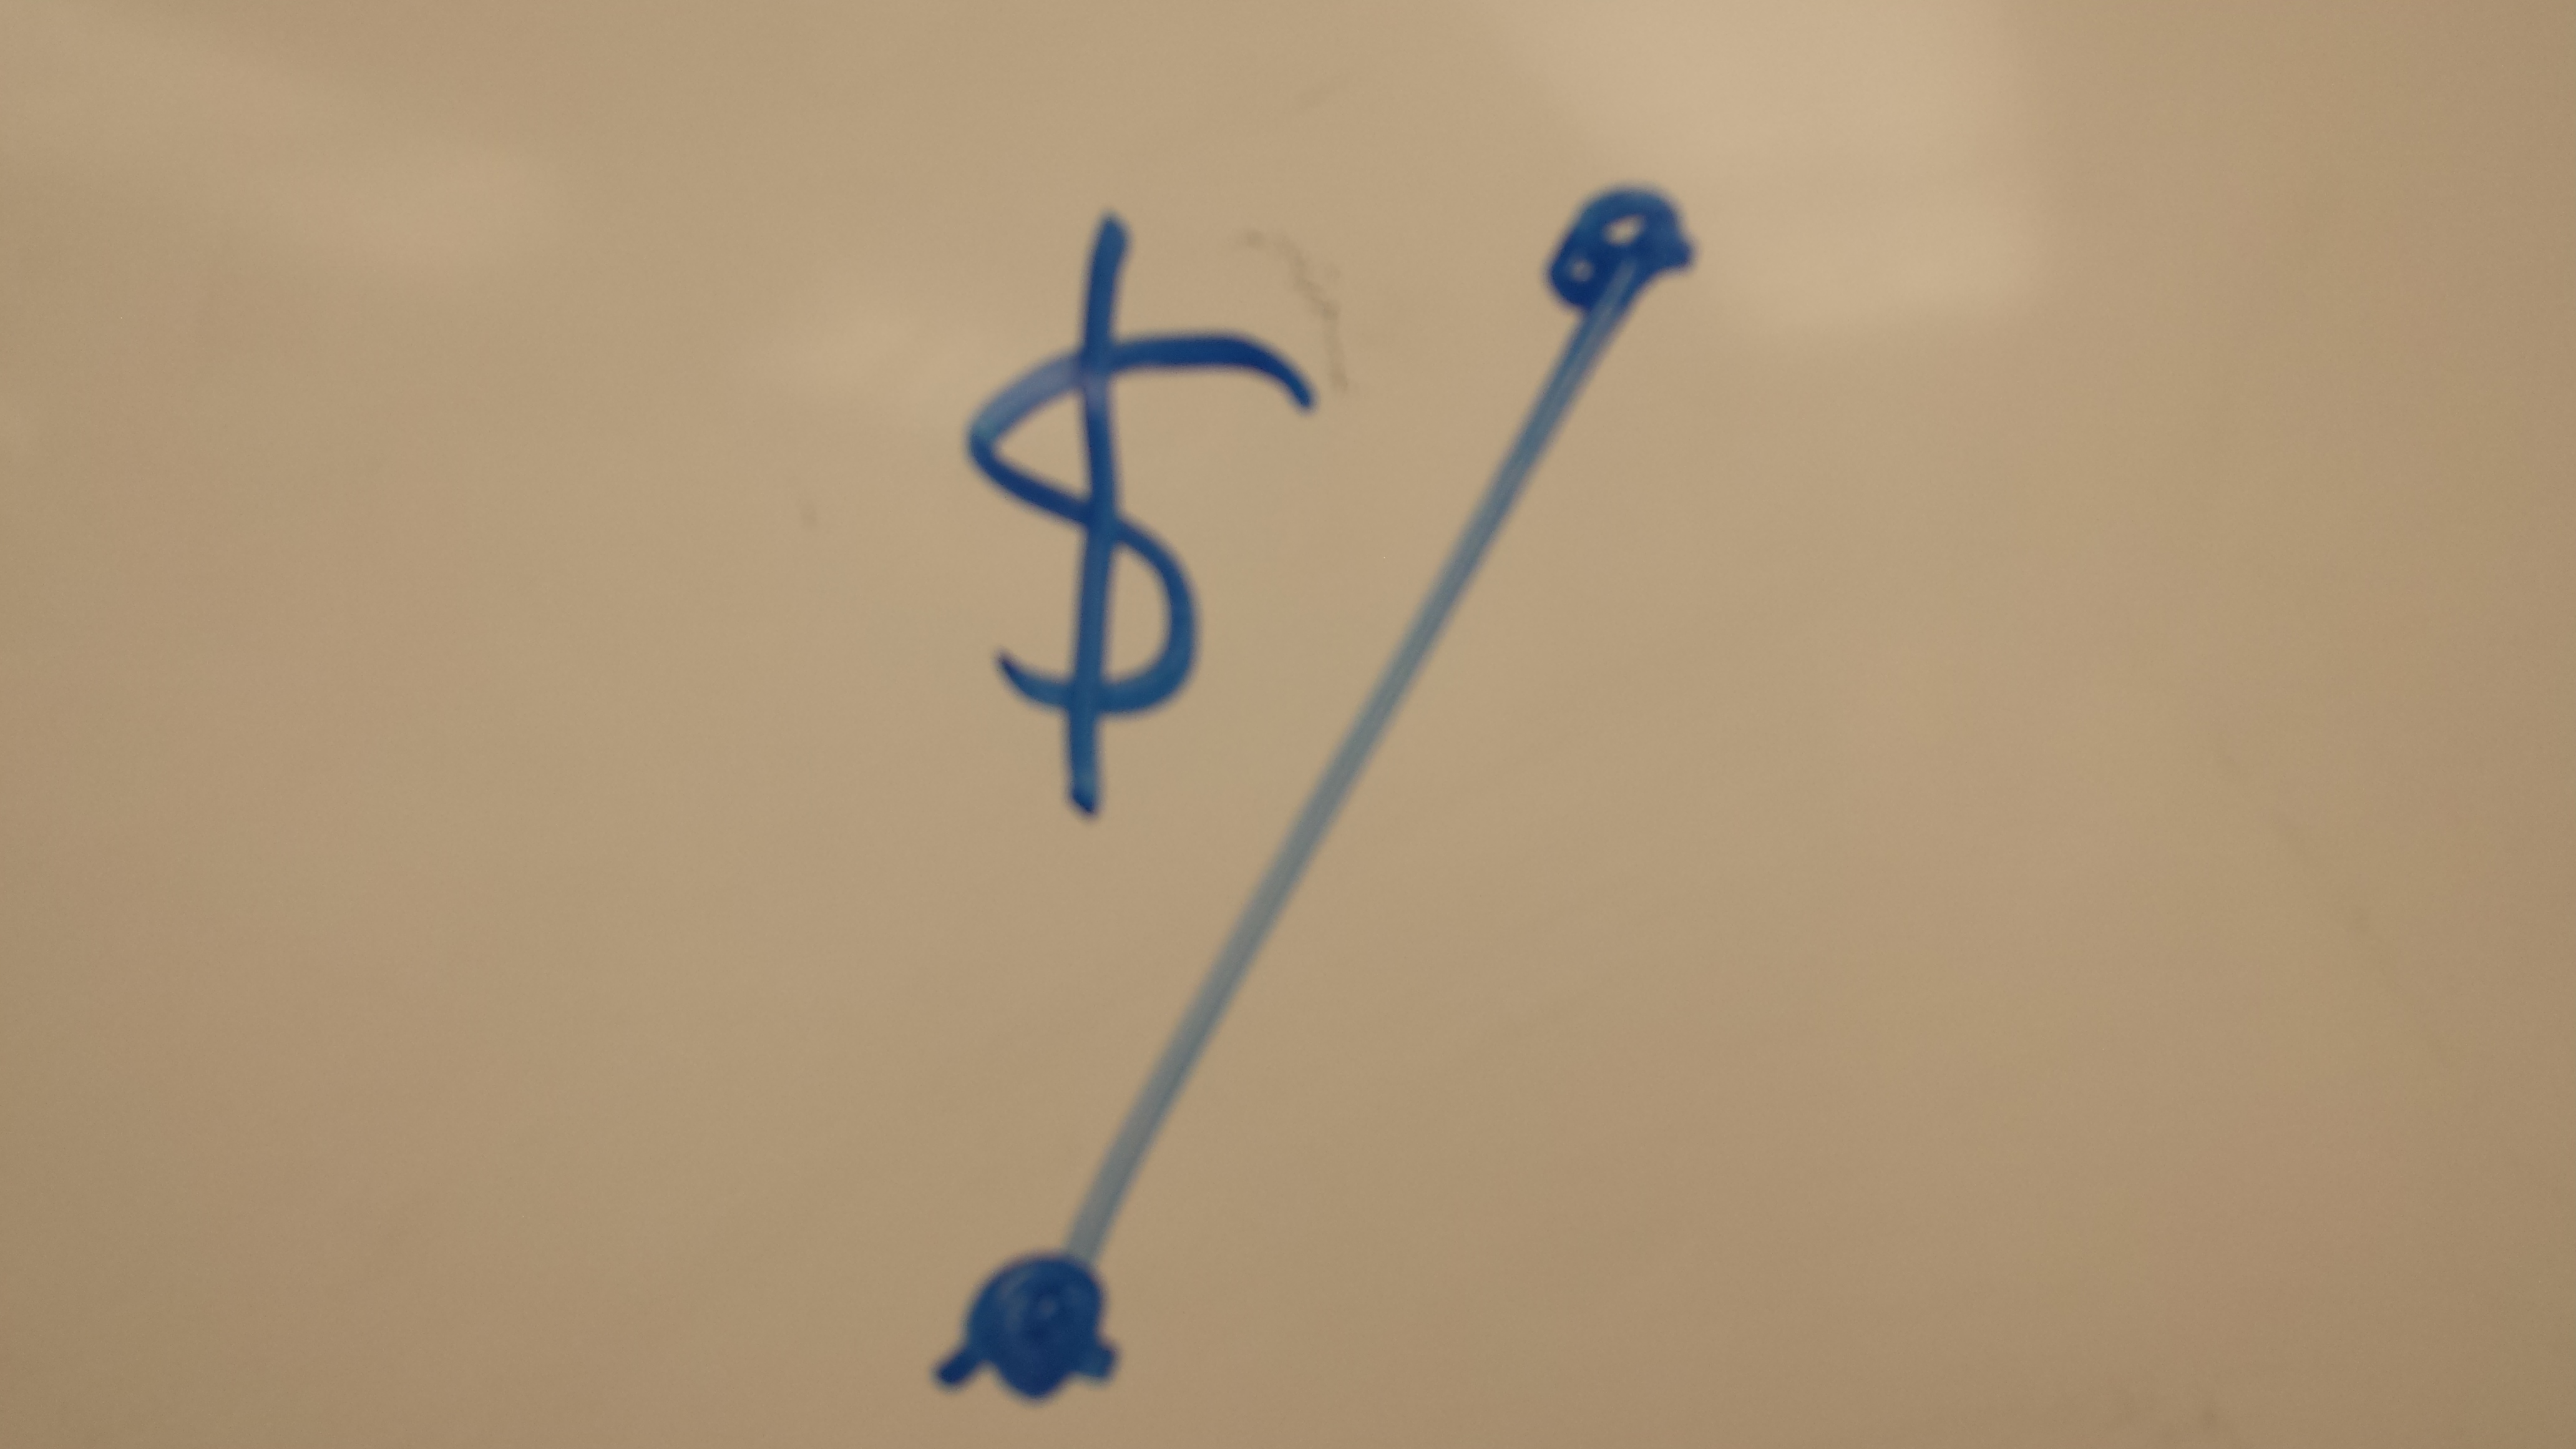
\includegraphics[width=90mm]{suffix_tree_a.jpg}
\caption{The suffix tree for the empty string concatenated with a dollar sign.  \label{overflow}}
\end{figure}

\item[] 

\begin{figure}[ht!]
\centering
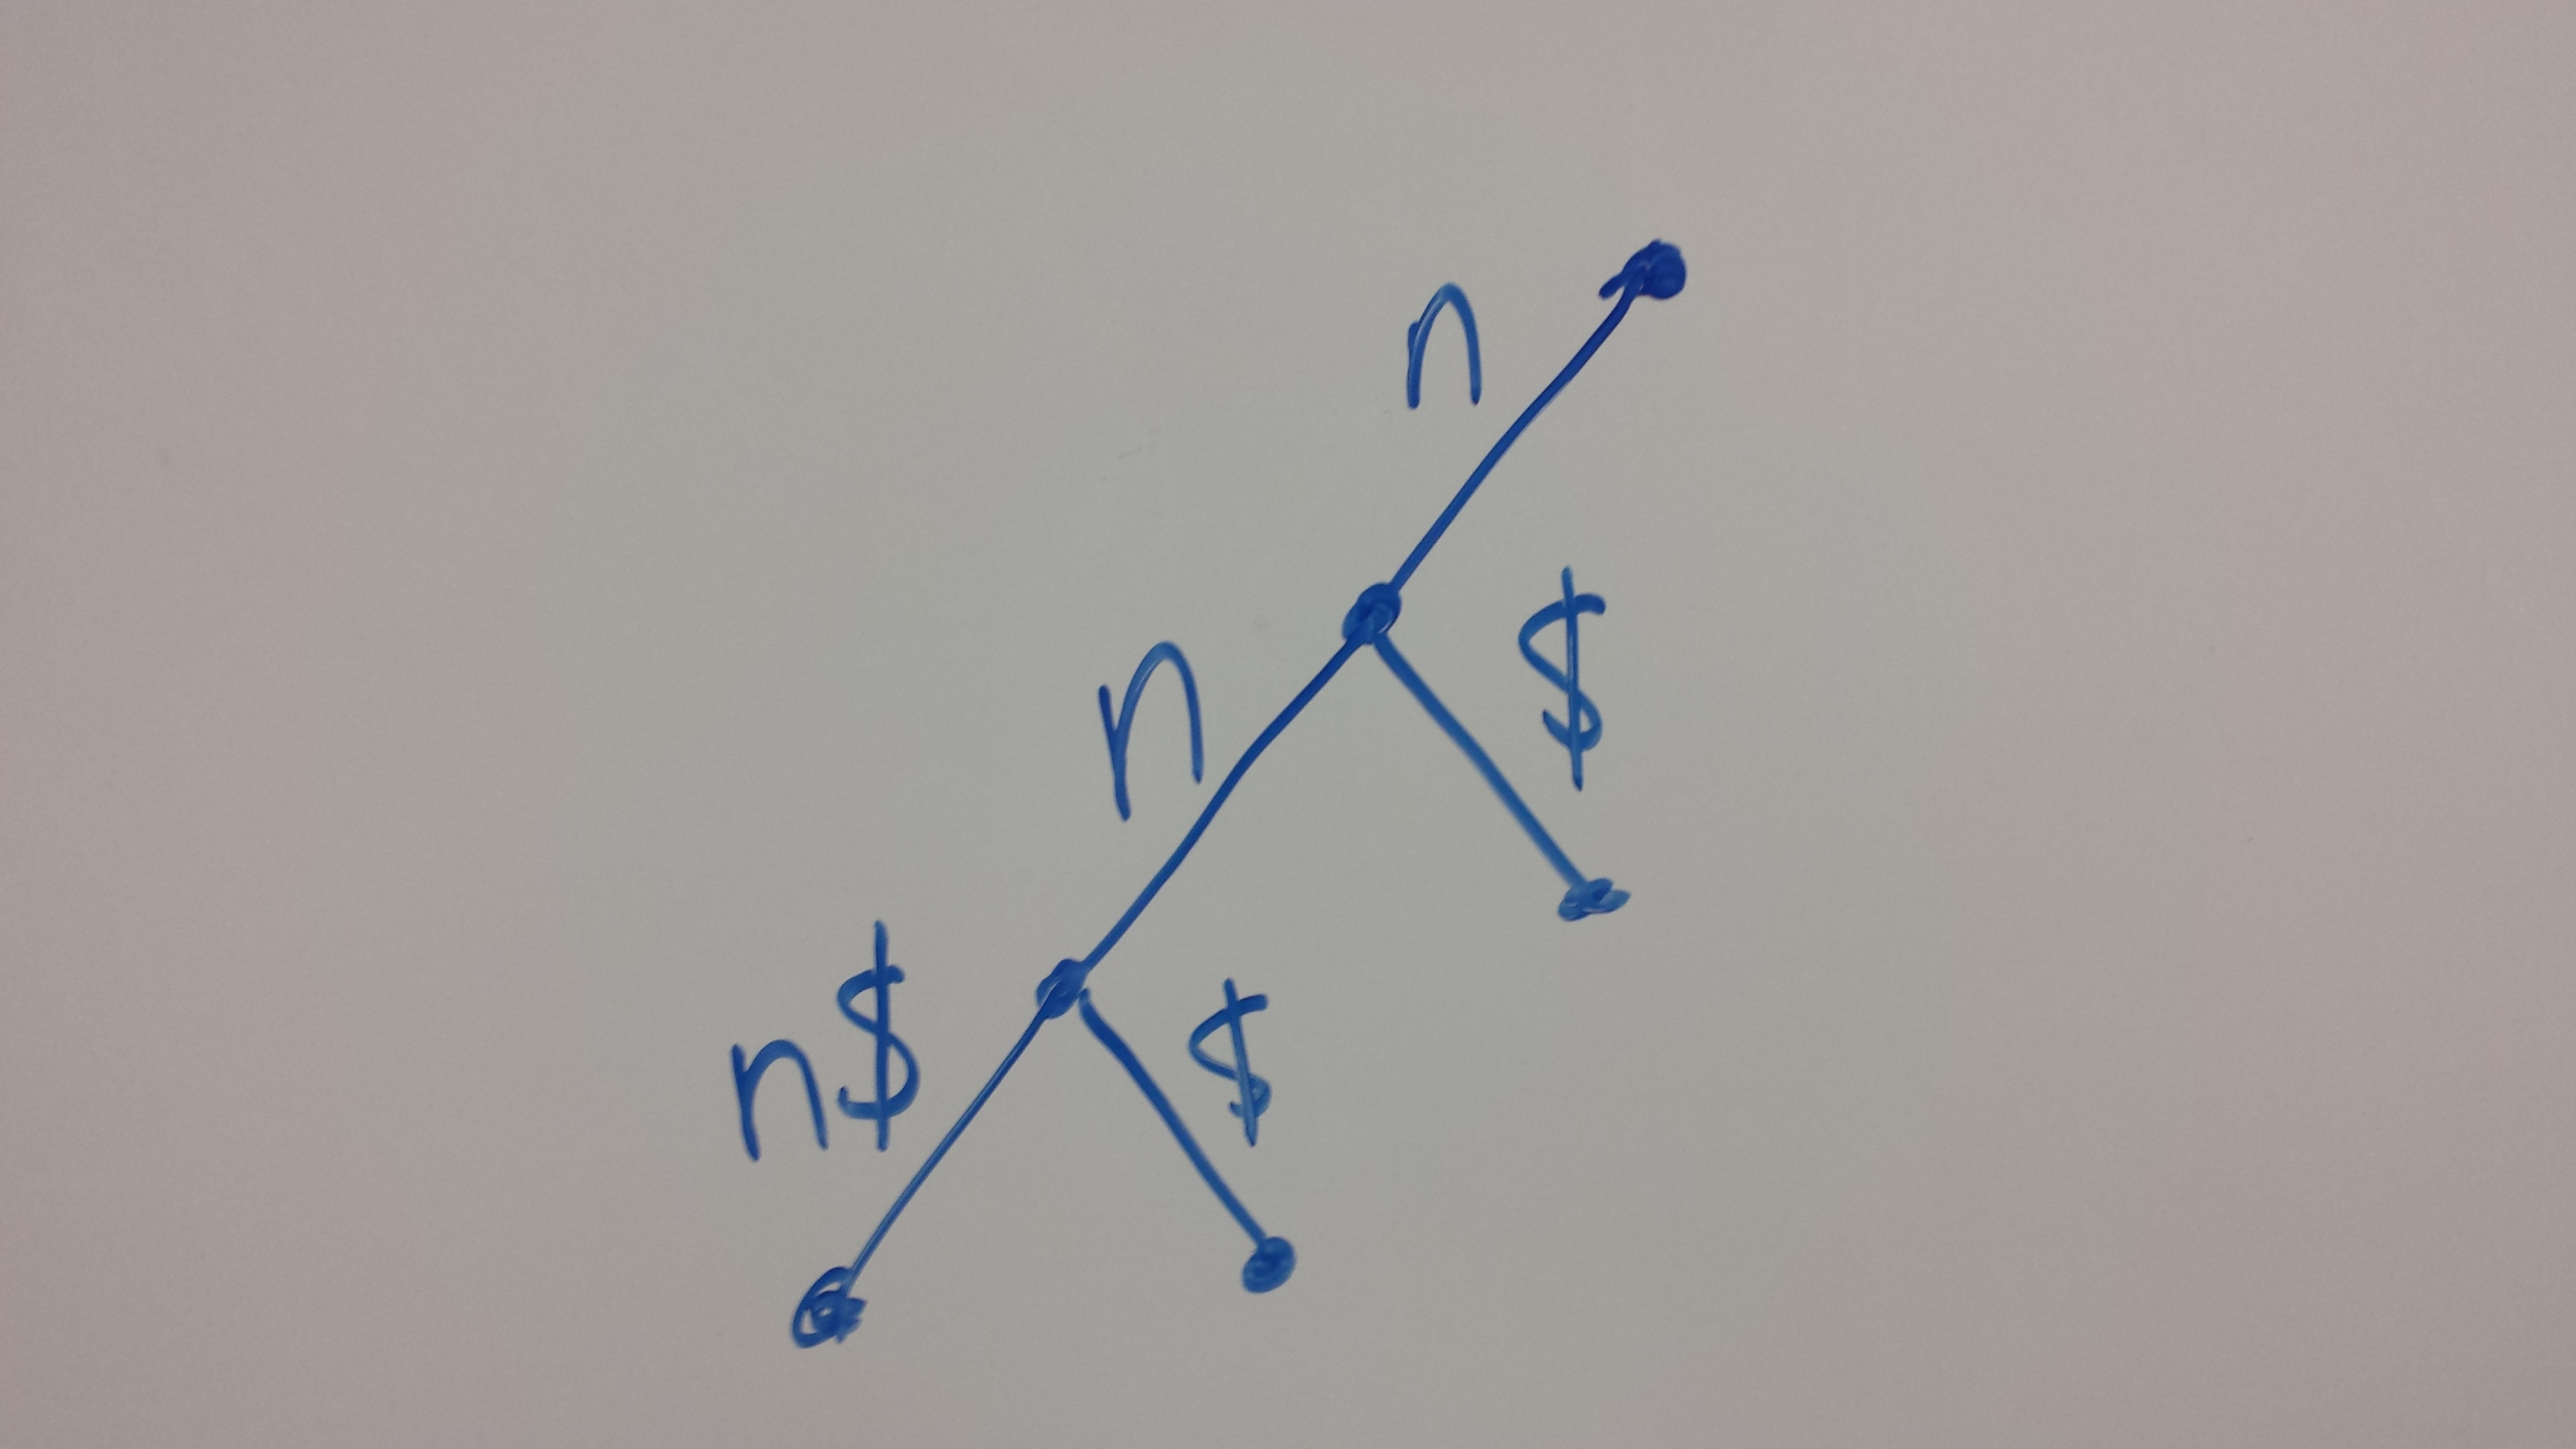
\includegraphics[width=90mm]{suffix_tree_b1.jpg}
\caption{The suffix tree for the string nnn(dollar), featuring edge label n(dollar) of length n/2.  \label{overflow}}
\end{figure}

\end{enumerate}

\bigskip
\bigskip

\noindent PROBLEM 2

\bigskip

\begin{enumerate}

\item[]  

\begin{figure}[ht!]
\centering
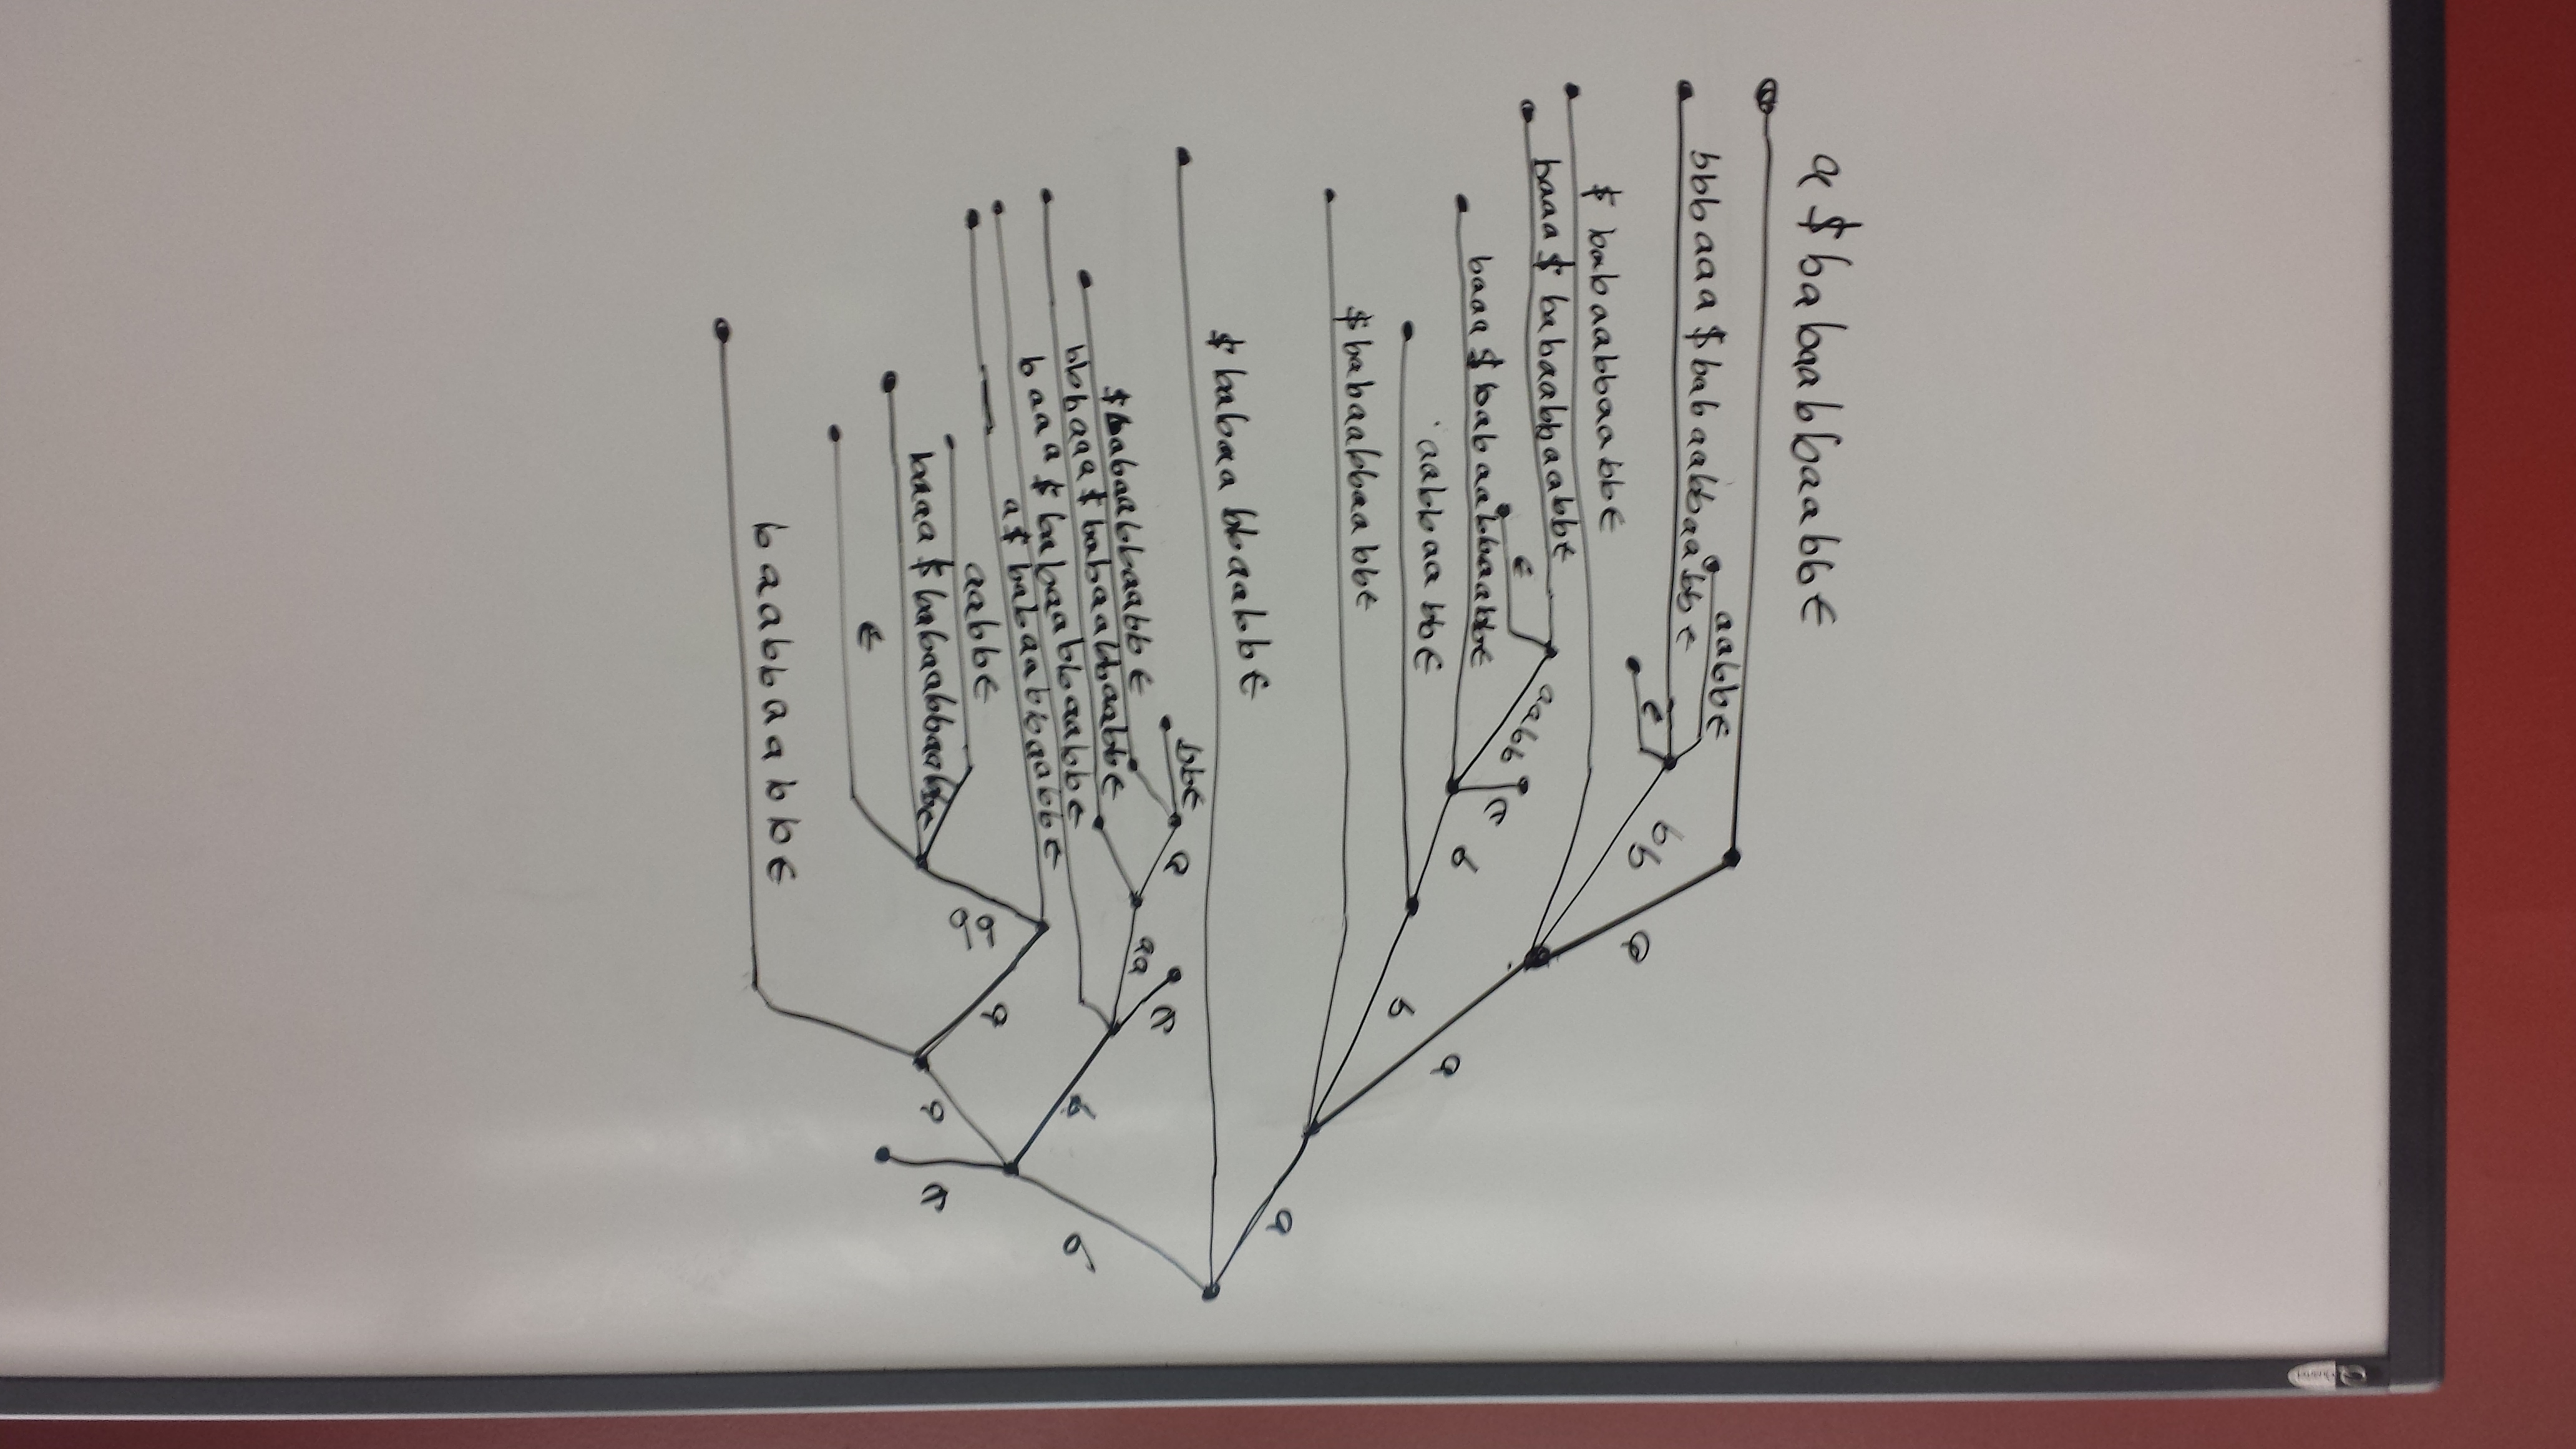
\includegraphics[width=90mm]{suffix_tree_2.jpg}
\caption{The longest substring is ``abbaabb''.  \label{overflow}}
\end{figure}

\item[] Tree is upside-down, sorry.


\end{enumerate}

\bigskip
\bigskip

\noindent PROBLEM 3

\begin{enumerate}
\item[a)] I don't know
\item[b)] I don't know
\item[c)] I don't know
\end{enumerate}

\end{document}